% Newton-Raphson tangent-line construction for notebook 04.
% f(x) = x^2 - 2; each tangent's x-intercept is the next iterate, marching
% x0 -> x1 -> x2 toward the root x* = sqrt(2).
% Standalone: compiles with `lualatex newton_raphson.tex`; loaded via render_tikz_file.
\documentclass[tikz,border=4pt]{standalone}
\usepackage{amsmath}
\usepackage{amssymb}
\usepackage{pgfplots}
\pgfplotsset{compat=1.18}
\usetikzlibrary{arrows.meta,calc}
\begin{document}
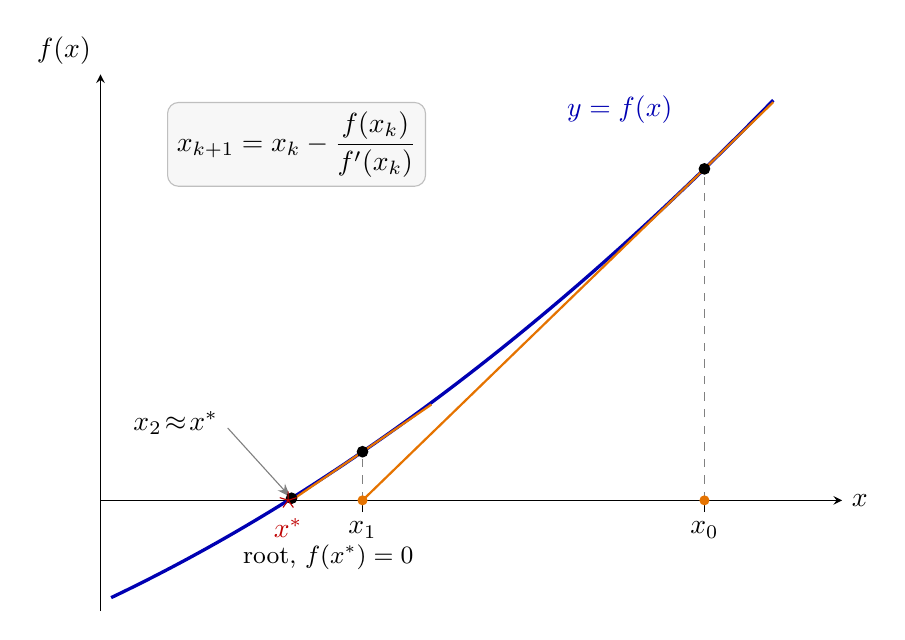
\begin{tikzpicture}[>=Stealth]
\begin{axis}[
    width=11cm, height=8.4cm,
    axis x line=middle, axis y line=left,
    xlabel={$x$}, ylabel={$f(x)$},
    every axis x label/.style={at={(ticklabel* cs:1.0)}, anchor=west},
    every axis y label/.style={at={(ticklabel* cs:1.0)}, anchor=south east},
    xmin=1.06, xmax=2.46, ymin=-0.95, ymax=3.65,
    xtick={1.55455, 2.2}, xticklabels={$x_1$, $x_0$},
    ytick=\empty,
    tick style={black}, tick align=outside,
    clip=false,
]

  % --- the curve f(x) = x^2 - 2 ---
  \addplot[domain=1.08:2.33, samples=120, blue!70!black, very thick] {x^2 - 2};
  \node[blue!70!black] at (axis cs:2.04,3.35) {$y=f(x)$};

  % --- tangent at x0 (intercept -> x1) ---
  \addplot[orange!90!black, thick] coordinates {(1.55455,0) (2.33,3.412)};
  % --- tangent at x1 (intercept -> x2) ---
  \addplot[orange!90!black, thick] coordinates {(1.42055,0) (1.68455,0.8208)};

  % --- vertical drop lines from the curve down to each iterate ---
  \draw[gray, dashed] (axis cs:2.2,0)     -- (axis cs:2.2,2.84);
  \draw[gray, dashed] (axis cs:1.55455,0) -- (axis cs:1.55455,0.41661);

  % --- points where the tangents touch the curve ---
  \addplot[only marks, mark=*, mark size=1.9pt, black]
    coordinates {(2.2,2.84) (1.55455,0.41661) (1.42055,0.01796)};

  % --- iterates on the axis ---
  \addplot[only marks, mark=*, mark size=1.6pt, orange!90!black]
    coordinates {(2.2,0) (1.55455,0)};

  % --- the root x* = sqrt(2) ---
  \addplot[only marks, mark=star, mark size=3.2pt, red!75!black]
    coordinates {(1.41421,0)};
  \node[red!75!black, anchor=north] at (axis cs:1.41421,-0.07) {$x^{*}$};
  \node[anchor=north] at (axis cs:1.49,-0.30)
    {\small root, $f(x^{*})=0$};

  % --- the x2 iterate label (essentially on the root) ---
  \draw[->, gray] (axis cs:1.30,0.62) -- (axis cs:1.4180,0.03);
  \node[anchor=east] at (axis cs:1.30,0.66) {$x_2\!\approx\!x^{*}$};

  % --- the update rule ---
  \node[draw=black!25, rounded corners, fill=black!3, align=center]
    at (axis cs:1.43,3.05)
    {$x_{k+1}=x_k-\dfrac{f(x_k)}{f'(x_k)}$};

\end{axis}
\end{tikzpicture}
\end{document}
